\chapter{基于代码依赖紧密度分析改进需求可追踪性生成方法}

\section{引言}

需求可追踪性是指,在软件生命周期中,对某一特定需求形成以及演变的追踪能力\cite{gotel1994analysis}。在软件维护和演化的过程中,需求可追踪性能够追踪一个需求使用期限的全过程以辅助利益相关者完成相应的软件活动\cite{mader2012assessing}。例如,需求到代码间的追踪关系能够帮助利益相关者进行代码变更的影响性分析,以维护需求和代码的一致性。然而,在实际的软件系统中,通常存在大规模的追踪关系,且软件实体(尤其是代码)变更频繁,导致追踪关系难以建立\cite{burgstaller2010understanding}。

为了减少生成追踪关系的人工成本,领域内已有工作集中于提高追踪关系的自动化程度。目前,信息检索技术被广泛用于解决追踪关系的生成问题\cite{antoniol2002recovering,cleland2005utilizing,marcus2003recovering}。一般的,基于信息检索的追踪关系生成方法利用信息检索模型(如VSM,JS与LSI)计算软件实体间(如需求与代码)的文本相似性,以自动化生成候选追踪关系列表,减少了实体间潜在关联的搜索空间。然而,以需求与代码为例,基于信息检索方法的效果严重依赖与需求与代码的文本质量,词汇失配(Vocabulary Mismatch)问题难以避免。为了解决这一问题,已有工作从提供额外的信息源(提交日志,缺陷修复报告,邮件列表)\cite{ali2013trustrace},为代码中不同来源的信息赋权\cite{ali2012empirical},考虑代码所有者上下文\cite{diaz2013using}等方面着手,以提高基于信息检索的追踪关系生成方法的精度。

同时,另一类工作关注于结合代码的文本信息与结构依赖应用于需求可追踪性生成及类似的领域,如特征定位\cite{zhao2006sniafl},概念分配\cite{scanniello2015link}。此类方法首先基于信息检索技术生成初始的候选追踪关系,并基于代码依赖关系的分析对已有候选追踪关系进行过滤或重排序。近期工作通过对代码依赖的进阶分析(利用PageRank算法\cite{scanniello2015link}),结合代码依赖与用户反馈\cite{panichella2013and}等方式提高了检索的精度。然而,上述工作在分析代码依赖关系时,认为所有的代码依赖关系是同样重要的,没有对各个依赖关系的重要性加以区分,从而无法充分发挥代码依赖关系的作用。

本章中,我们提出了一种代码依赖关系的紧密度分析方法以量化代码类之间依赖的交互程度。同时,基于代码关系的紧密度分析,我们提出了一种改进的需求到代码间追踪关系的生成方法TRICE(Traceability Recovery based on Information retrieval and ClosEness analysis)

\section{背景}
在本节,我们将说明本工作的研究动机,并给出我们的问题定义。

\subsection{研究动机}

在本小节,我们将给出一个具体的示例以解释我们的研究动机。

在医疗数据管理系统iTrust中,存在类\emph{MonitorAdverseEvents}。观察代码发现,类\emph{MonitorAdverseEvents}分别与\emph{MonitorAdverseEventAction},\emph{AuthDAO}存在调用依赖,\emph{MonitorAdverseEvents}与前者间存在三个不同的函数调用,与后者间只存在一个函数调用。此外,\emph{MonitorAdverseEventAction}只被\emph{MonitorAdverseEvents}调用,而\emph{AuthDAO}还被其它类所调用。比较这两种依赖关系,我们发现到\emph{MonitorAdverseEvents}与\emph{MonitorAdverseEventAction}之间有更强的交互,暗示着它们之间的依赖关系更紧密。类似的观察已经作为启发式规则应用于重构中类的自动提炼\cite{bavota2014automating}。

在软件系统中,一个需求通常是由代码中的若干类共同协作实现的。因此,如果两个类之间的依赖关系较为紧密(有较强的交互),则它们在功能上可能具有较高的相似性。在生成需求到代码间的追踪关系时,对代码依赖关系的紧密度分析可以发现与需求文本相似性低,但与相关类依赖关系紧密的类,以达到提高检索精度的目的。

\subsection{问题定义}
在本节,我们将定义基于代码依赖关系紧密度分析改进需求可追踪性生成方法的问题。

\textbf{\emph{问题定义.}} \emph{给定一个需求集合$R$,该需求集合包含$m$个需求文本,同时给定代码集合$C$,包含$n$个类,且类之间存在依赖关系(如调用依赖,数据依赖)。基于信息检索的需求到代码间追踪关系生成方法能够建立候选追踪关系列表$T = \{t_{1}, \cdots, t_{n}\}$,$t_{i}$为一个三元组$(req, class, score)$,其中$req \in R$,$class \in C$,$score$表示需求与代码类的相似度得分,列表$T$中的追踪关系根据相似性得分倒序排列。问题是:分析代码依赖关系的紧密度是否能够提高追踪关系生成方法的精度。}

\section{方法概述}
在本节,我们将介绍基于代码依赖紧密度分析的需求可追踪性生成改进方法TRICE。TRICE的过程包括以下四个步骤:(1)代码类间的依赖关系捕获与组织;(2)计算代码依赖关系的紧密度,并生成相应的图结构CDCGraph(Code Dependencies Graph with Closeness);(3)基于信息检索技术生成需求到代码的候选追踪关系;(4)利用代码依赖关系的紧密度分析,对候选追踪关系进行重排序。我们将在后续四个小节对以上步骤进行详细阐述,并辅以iTrust中一个实际的例子来说明相关概念。

\section{代码类间的依赖关系捕获与组织}
在本章工作中,我们考虑了以下四种类间的依赖关系,并辅以iTrust代码片段进行说明。

\begin{enumerate}
  \item 调用依赖:如果两个类之间存在一个调用依赖,则表示两个类之间至少有一个函数调用。由于类\emph{MonitorAdverseEventAction}中调用了\emph{EmailUtil}的函数\emph{sendEmail()},因此类\emph{MonitorAdverseEventAction}与\emph{EmailUtil}存在调用依赖。
  \item 使用依赖:如果一个类使用了另一个类的对象,则表示两个类之间存在使用依赖。故类\emph{MonitorAdverseEventAction}与\emph{EmailUtil}存在类的使用依赖。
  \item 继承依赖:表示两个类之间存在继承关系。
  \item 数据依赖:表示两个类之间读写了同样的数据内容\cite{kuang2015can}。观察图N可以发现,类\emph{MonitorAdverseEventAction}与\emph{EmailUtil}之间存在显式的调用依赖和使用依赖,但\emph{EmailUtil}与\emph{SendMessageAction}之间并没有显式的依赖关系。然而,函数\emph{SendMessageAction.saveReceiver()}与函数\emph{EmailUtil.sendEmail()}都传递了Email类型的对象作为参数,因此\emph{EmailUtil}与\emph{SendMessageAction}之间存在数据依赖。
\end{enumerate}

为了捕获上述代码依赖,我们选用基于JVMTI(Java Virtual Machine Tool Interface)的动态分析工具\cite{kuang2015can}以捕获函数间的调用及数据依赖。由于该工具是加载于JVM的运行时刻进行依赖捕获,并通过测试用例驱动执行,因此能够分析真实的代码执行时刻依赖,同时正确处理多态。

根据函数间的调用及数据依赖,我们可以衍生出上述类间的代码依赖。首先,类的调用依赖可以由类之间包含多少不同的函数调用(同方向的)来确定。其次,如果两个属于不同类的函数间存在数据依赖,则认为函数所属的类存在同样的数据依赖,类的使用依赖也由此确定。最后,由于子类会调用父类的构造函数,因此类的继承依赖可以从函数的调用依赖中获得。

由于类的调用依赖,使用依赖,继承依赖结构相似且有较大的重叠关系,因此我们将上述三种依赖统一表示为直接调用依赖。后续我们将介绍对类的直接调用依赖与数据依赖的紧密度计算方法。

\section{代码依赖关系的紧密度计算}

基于捕获的代码依赖关系,我们通过以下四个步骤计算代码依赖关系的紧密度,并生成相应的图结构CDCGraph。

\begin{enumerate}
  \item 建立代码依赖关系图(CDGraph):首先,我们定义代码依赖关系图CDGraph(Code Dependency Graph)为一个有序对$CDGraph = <V, E>$,其中$V$是代码中类的集合,$E$是代码依赖边的集合,其中,依赖边包括类的直接调用依赖与数据依赖。图N展示了iTrust系统示例的代码依赖关系图。其中,有方向的实线表示直接调用依赖,并标记了不同的函数调用或类的使用数量;无方向的虚线表示数据依赖,并标记了类之间共享数据类型的数量。

  \begin{figure}[thb]
    \centering
    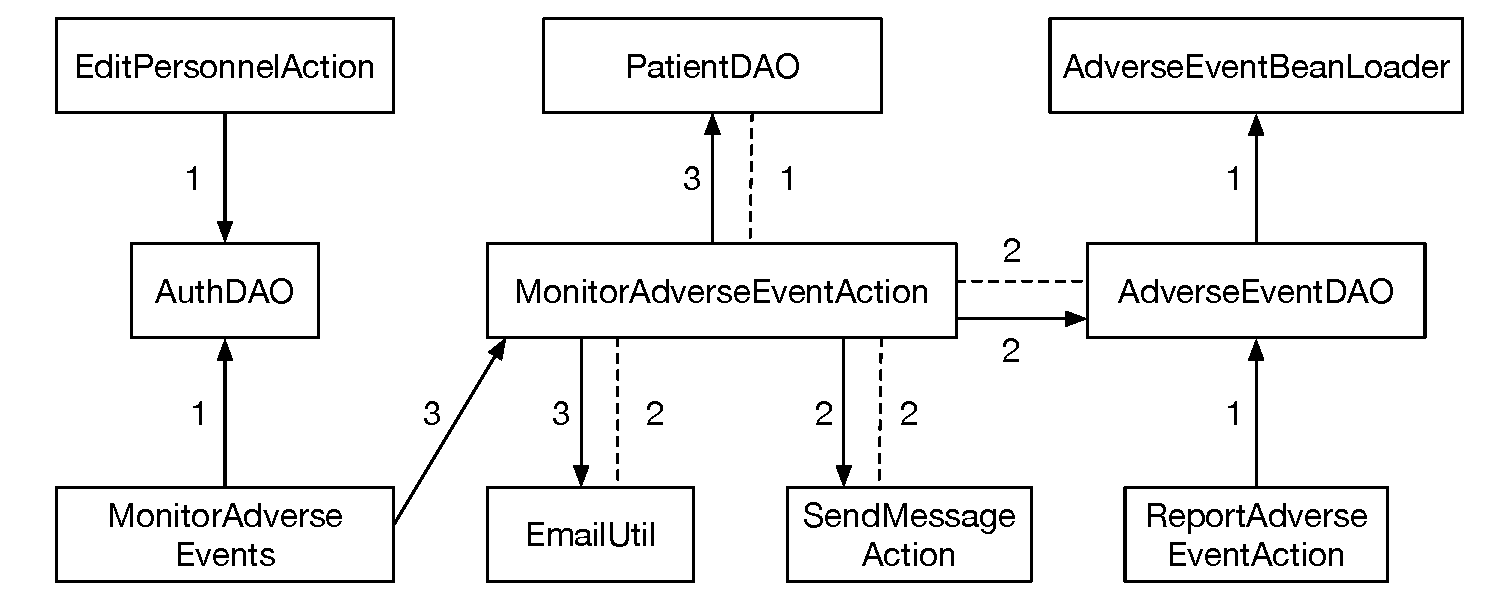
\includegraphics[width=0.8\textwidth]{./figures/traceability_sample/sample_weight.pdf}
    \caption{与日志记录、展示功能有关的部分函数及其依赖结构}
    \label{F:sample_weight}
  \end{figure}

  \item 直接调用依赖的紧密度计算:根据对研究动机中示例的观察,代码类之间的依赖关系表明了类之间的交互程度。在后文中,我们用源节点表示调用(使用)者,用目标节点表示被调用(使用)者。对于直接调用依赖而言,依赖的紧密程度可能与以下3点有关:(1)类之间包含多少不同的函数调用或类的使用;(2)源节点调用(使用)了多少其它的类,既源节点的出度;(3)目标节点被多少其它的类调用(使用),既目标节点的入度。 从直觉上理解,如果两个类之间存在较多种类的函数调用或类的使用,那么这两个类之间的交换较为紧密。同时,如果源节点的出度越小,且目标节点的入度越小,则表明源节点更专注于完成目标节点的任务,目标节点也更专注于服务源节点。基于上述两点观察,我们定义类间直接调用依赖的紧密度计算公式如下:

  \begin{align}Closeness_{call}=\frac {2N} {WeightedOutDegree_{e.source}+WeightedInDegree_{e.target}}\end{align}

  其中,$N$表示两个类之间依赖边上不同的函数调用与类的使用的数目,$WeightedOutDegree_{e.source}$表示源节点的出度,$WeightedInDegree_{e.target}$表示目标节点的入度,并用每一条直接调用依赖边上,不同的函数调用与类的使用的数目,来表示出入度的权重。

  \item 数据依赖的紧密度计算:数据依赖关系表明两个类之间共享了某些类型的数据。在计算数据依赖的紧密度之前,我们首先需要过滤与通用数据类型有关的数据依赖。在iTrust系统中,DAOFactory作为与数据库交互的工具类,它被系统中的绝大多数类所访问。这些类相互之间虽然存在关于DAOFactory的数据依赖,但这样的数据依赖由于DAOFactory过于通用,无法用于分析类之间的紧密度分析。因此,我们引入一种数据类型的权重计算方式IDTF(Inverse Data Type Frequency)\cite{kuang2015can}:

  \begin{align}IDTF=\log\frac {N} {n_{dt}}\end{align}

  其中,N表示数据依赖的总数,ndt表示给定的数据类型在所有数据依赖中出现的次数。我们通过设置阈值T-idtf的方式,过滤IDTF值在阈值以下的数据类型和基于此类数据类型的数据依赖。与信息检索中的IDF概念类似,IDTF反映了一个数据类型在系统整个代码中的全局重要性。IDTF值越高,表示该数据类型越独特,如果两个类有关于该数据类型的数据依赖,则表明类之间的交互也较强。除此以外,如果两个类还分别与其它类存在数据依赖,则会降低两个类之间数据依赖的本地重要性。基于上述两点观察,我们定义类间数据依赖的紧密度计算公式如下:

  \begin{align}Closeness_{data}=\frac {\sum _{x \in \{DT_{i}\cap DT_{j}\}}IDTF(x)} {\sum _{y \in \{DT_{i}\cup DT_{j}\}}IDTF(y)}\end{align}

  其中,$IDTF(x)$表示数据类型$x$的IDTF值,$DT_{i}$与$DT_{j}$分别表示两个类所有数据依赖边的数据类型。

  \item 生成CDCGraph:基于上述三个步骤,我们定义CCDGraph(Code Dependency Graph with Closeness)为一个有序对$CCDGraph = <V, E>$,其中$V$是代码中类的集合,$E$是代码依赖边的集合,其中,依赖边包括类的直接调用依赖与数据依赖,前者依赖边的权重为直接调用依赖的紧密度值,后者依赖边的权重为数据依赖的紧密度值。由图N衍生而来,图N展示了iTrust系统示例的CDCGraph。

  \begin{figure}[thb]
    \centering
    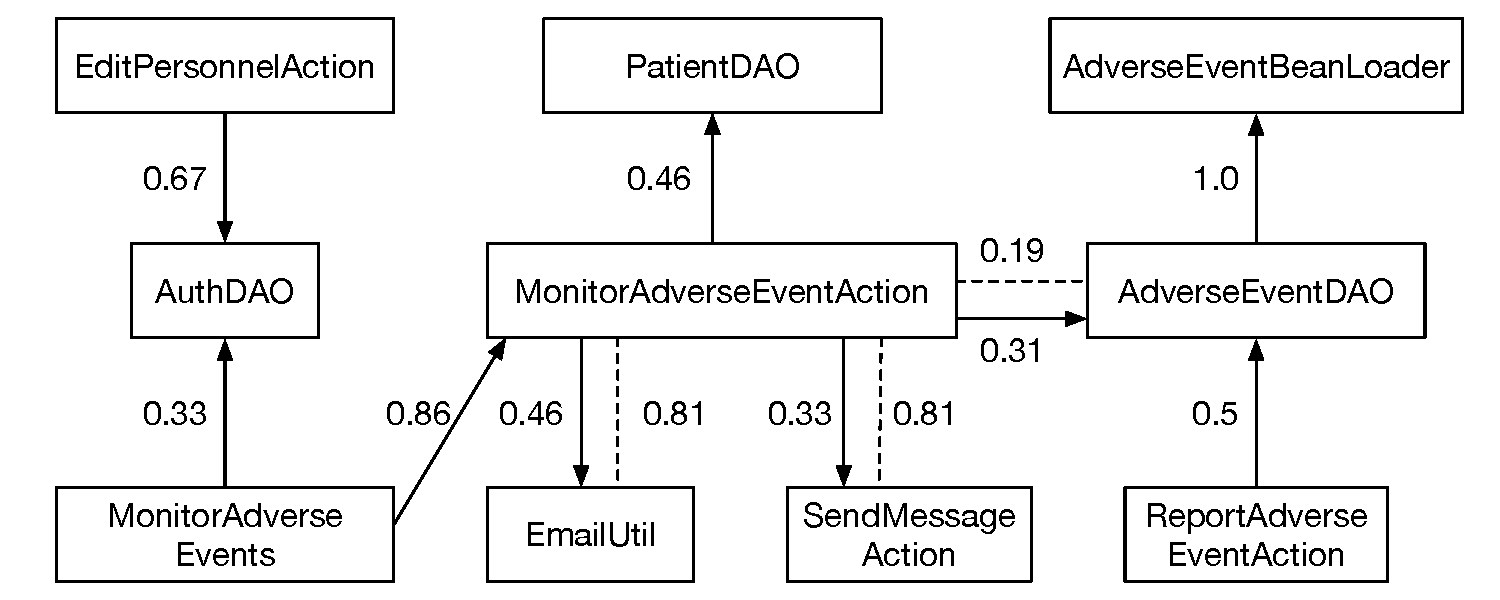
\includegraphics[width=0.8\textwidth]{./figures/traceability_sample/sample_closeness.pdf}
    \caption{与日志记录、展示功能有关的部分函数及其依赖结构}
    \label{F:sample_closeness}
  \end{figure}
\end{enumerate}

\section{生成需求到代码的候选追踪关系}

\begin{enumerate}
  \item 生成语料库:对于代码中的每一个类,我们抽取其类名,类的注释,函数名,函数的注释,域名等信息作为代码的文本。对于每一个需求(如用例),我们抽取需求的标题及内容(在用例中,一般包括前提,主流程,子流程等)作为需求文本。
  \item 标准化语料库:对于代码的文本,我们首先根据代码标识符的命名规则(驼峰命名法,下划线分割命名法),将标识符分隔为若干独立词项。然后,对需求和代码文本进行统一的预处理操作以标准化文本,预处理过程包括去停用词,词形还原和词根提取等。
  \item 索引语料库并计算相似度:我们利用TF-IDF计算词项的权重并建立索引,在计算需求文本与代码文本时,我们使用了三个不同的检索模型:VSM\cite{antoniol2002recovering},LSI\cite{marcus2003recovering}与JS\cite{abadi2008traceability}。
  \item 生成候选追踪关系列表:对于每个需求,将代码按相似度值倒序排列,生成候选追踪关系列表。
\end{enumerate}

\section{基于代码依赖关系紧密度的追踪关系重排序}
在本节,我们的目的在于基于代码依赖关系改进候选追踪关系的排序。我们的想法源于以下两点观察:(1)对于给定的一个需求,候选追踪关系中IR值最高的类通常与该需求有关(2)对于给定的一个需求,实现该需求的代码通常是相互关联的,形成关联的需求域\cite{burgstaller2010understanding},而不是分散的。基于上述两点观察,我们提出了基于代码依赖关系紧密度分析的追踪关系重排序方法,包括以下两个步骤:(1)建立初始需求域,并提升初始域内所有的类;(2)对于初始域外的类,根据它们与域内类的代码依赖关系,给这些初始域外类的IR值以奖励。以下我们将具体阐述每个步骤。

\subsection{建立初始需求域}
我们给定阈值$T_{call}$与$T_{data}$,以对CDCGraph进行剪枝,删去紧密度值小于$T_{call}$的直接调用依赖边与紧密度值小于$T_{data}$的数据依赖边。剪枝后CDCGraph中的依赖边表明较为紧密的依赖关系。对于给定的一个需求,我们选取候选追踪关系中IR值最高且存在依赖邻居(直接调用依赖或数据依赖)的类作为建立初始需求域的种子类,如果IR值最高的类没有依赖邻居,则依次寻找次高IR值的类。然后,我们基于CDCGraph引入与种子类依赖关系紧密的其他类,以建立初始域。在此过程中,对于两种不同的代码依赖关系,我们使用了两种不同的策略。在剪枝后的CDCGraph中,对于直接调用依赖,我们将种子类所处调用链中的其他类加入初始域;对于数据调用依赖,我们将种子类的直接邻居类加入初始域。对这些因为与种子类存在依赖关系,而被加入初始域的类,我们将其IR值提升至与种子类相同的IR值。我们建立初始需求域的具体算法如下:

\begin{algorithm}[htbp]
\caption{Establishing Initial Region}
\label{alg:EstablishingInitialRegion}
initialRegion $\leftarrow$ $\emptyset$;\\
prunedGraph $\leftarrow$ CDCGraph.setPruning($T_{call}$,$T_{data}$);\\
topLink $\leftarrow$ candidateList.next();\\
\While{prunedGraph.hasNoNeighbors(topLink.class)} {
  initialRegion.add(topLink.class);\\
  topLink $\leftarrow$ candidateList.next();
} 
initialRegion.add(topLink.class);\\
initialRegion.topIRValue $\leftarrow$ topLink.IRValue;\\
reachedClasses $\leftarrow$ $\emptyset$;\\
reachedClasses.add(prunedGraph.getTransitiveCallers(topLink.class));\\
reachedClasses.add(prunedGraph.getTransitiveCallees(topLink.class));\\
reachedClasses.add(prunedGraph.getNeighborsByData(topLink.class));\\
\ForEach {link in candidateList}
{
    \If {reachedClasses.contains(link.class)} {
      link.IRValue $\leftarrow$ initialRegion.topIRValue;\\
      initialRegion.add(link.class);
    }
}
candidateList.reorderByIRValue();\\
\end{algorithm}

\subsection{重排序初始域外的追踪关系}
在建立初始域之后,我们分析初始域外类与域内类的代码依赖关系,以给予这些初始域外类的IR值奖励。类似于建立初始域的过程,我们为直接调用依赖与数据依赖设计了两种不同的策略。

对于直接调用依赖,假设初始域外的类为$C_{out}$,初始域内的类为$C_{in}$,我们在CDCGraph中寻找$C_{out}$与$C_{in}$之间的有效路径。一条有效路径需要满足以下两个条件:(1)路径中的边必须是同向,指可以迭代地访问$C_{out}$的调用节点(或被调用节点)以到达$C_{in}$;(2)路径中包含的节点只有一个(既$C_{in}$)在初始域内(为了避免重复)。如果这样的有效路径存在,则我们计算路径中直接调用依赖边紧密度值的几何平均值,并根据如下公式更新$C_{out}$的IR值:

\begin{align}IR_{call}=IR_{origin}+(IR_{top}-IR_{origin})^{\left| PATH\right|}\sqrt {\prod _{x \in PATH}Closeness_{call}(x)} \end{align}

其中,$IR_{origin}$表示$C_{out}$原有的IR值,$IR_{top}$表示初始域中种子类的IR值,$Path$表示$C_{out}$与$C_{in}$间路径的依赖边集合,并用$Closeness_{call}(x)$表示路径中直接调用依赖边$x$的紧密度值。需要注意的是,$C_{out}$与$C_{in}$间可能存在多条路径,此时我们只选取使$C_{out}$的IR值增幅最大的路径。

对于数据调用依赖,如果初始域外的类$C_{out}$为初始域内的类$C_{in}$的直接邻居,则基于数据依赖的紧密度值更新$C_{out}$的IR值,公式如下:

\begin{align}IR_{call}=IR_{origin}+(IR_{top}-IR_{origin})Closeness_{data}(x) \end{align}

其中,其中,$IR_{origin}$表示$C_{out}$原有的IR值,$IR_{top}$表示初始域中种子类的IR值,$Closeness_{data}(x)$表示$C_{out}$与$C_{in}$间数据依赖边的紧密度值。

基于直接调用依赖(或数据依赖),如果初始域外的类$C_{out}$到多个初始域内的类都存在有效路径(或为多个初始域内类的直接邻居),则$C_{out}$的IR
值可以被多次奖励。此外,$C_{out}$的IR值可以同时获得来自直接调用依赖和数据依赖的奖励,但是IR值提升的上限不能超过初始域内种子类的IR值。基于代码依赖关系紧密度重排序追踪关系的算法如下:
\begin{algorithm}[htbp]
\caption{Re-rank Links outside Initial Region}
\label{alg:Re-rankLinksOutsideInitialRegion}
topIRValue $\leftarrow$ initialRegion.topIRValue;\\
\ForEach {link in candidateList} {
	\If {!initialRegion.contains(link.class)} {
   		\ForEach {c in initialRegion} {
        	pathList $\leftarrow$ findValidPaths(link.class, c);\\
          	$gMean$ $\leftarrow$ 0;\\
          	\ForEach {path in pathList} {
            	$gMean$ $\leftarrow$ max(GeometricMean($Closeness_{call}$(path)), $gMean$);
          	}
          	link.IRValue $\leftarrow$ link.IRValue + $gMean$(topIRValue - link.IRValue);\\
           	\If {hasDataDependencies(c, link.class)} {
            	link.IRValue $\leftarrow$ link.IRValue + $Closeness_{data}$(c, link.class)(topIRValue - link.IRValue);
          	}
      	}
      	\If {link.IRValue \textgreater \ topIRValue} {
       		link.IRValue $\leftarrow$ topIRValue;
        }
    }
}
candidateList.reorderByIRValue();
\end{algorithm}

\section{实验与分析}
在此小节,我们通过实验以验证TRICE的有效性。接下来,将具体阐述我们的实
验设置及实验结果与分析。

\subsection{实验系统及IR模型}
我们的实验在三个真实的中量级软件系统上进行:iTrust,GanttProject与jHotDraw。表N列举这三个系统的基本信息。这些系统都提供有效的需求规约,更重要的是,这些系统提供标准的需求到代码间的追踪关系(RTM),用于作为实验的Oracle。其中,iTrust在发布时就提供了需求到函数的RTM。对于jHotDraw与GanttProject,我们招募了系统的原开发者以建立高质量的需求到类的RTM。为了保持实验时RTM粒度的一致性,对于iTrust,我们由需求到函数的RTM衍生出需求到类的RTM(如果需求到某一个函数的追踪关系存在,那么需求到该函数所属类的追踪关系存在)。为了保证TRICE的泛化能力,我们选取了三个被广泛使用的IR模型,VSM,LSI与JS。

\begin{table}[]
\centering
\caption{My caption}
\label{my-label}
\begin{tabular}{@{}lccc@{}}
\toprule
           & iTrust & Gantt & jHotDraw \\ \midrule
版本         & 13.0   & 2.0.9 & 7.2      \\
编程语言       & Java   & Java  & Java     \\
千行代码(KLoC) & 43     & 45    & 72       \\
代码(类)      & 131    & 124   & 144      \\
需求(用例)     & 34     & 16    & 16       \\
调用依赖     & 274    & 452   & 691      \\
数据依赖       & 4844   & 1788  & 1815     \\
追踪关系       & 248    & 315   & 221      \\ \bottomrule
\end{tabular}
\end{table}

\subsection{评价指标}
为了验证不同追踪关系生成方法的表现,我们选用了信息检索中两个重要的指标Precision(准确率)与Recall(召回率):
\begin{align}recall=\dfrac {\left| correct\cap retrieved\right| } {\left| correct\right| }\% \end{align}
\begin{align}precision=\dfrac {\left| correct\cap retrieved\right| } {\left| retrieved\right| }\% \end{align}

其中$correct$表示正确的追踪关系(在Golden RTM中)集合,$retrieved$表示追踪关系生成方法所检索的追踪关系集合。一种常用的比较IR
方法的方式是,在不同的$Recall$水平比较方法间的准确率,可以由$Precision-Recall$曲线展示。为了进一步衡量追踪关系的整体质量,我们选用了信息检索中两个常用指标:$AP$(Average Precision)与$MAP$(Mean Average Precision)。其中,$AP$用于度量全部查询(需求)所检索的相关文档(追踪关系)的排序质量,计算方式如下:
\begin{align}
AP=\dfrac {\sum _{r=1}^{N}\left( Precision\left( r\right) \times isRelevant\left( r\right) \right) } {\left| RelevantDocuments\right| }
\end{align}

其中,$r$表示目标实体在列表中的排序,$N$表示文档的总数。$Precision(r)$表示在前$r$个时,列表的准确率。$isRelevant()$为一个二值函数,如果文档是相关的,则返回1,若无关,则返回0。同时,$MAP$用于度量不同查询(需求)所检索的相关文档(追踪关系)$AP$的平均值,计算方式如下:
\begin{align}
MAP=\dfrac {\sum _{q=1}^{Q}AP\left( q\right)} {q}
\end{align}
其中,$q$表示一次查询(需求),$Q$表示查询(需求)的总数。

\subsection{研究问题}
我们在x.x.x节定义了如下的研究问题:

Q:分析代码依赖关系的紧密度是否能够提高追踪关系生成方法的精度。

为了回答上述研究问题,我们将TRICE与三种基线方法进行比较:纯粹基于信息检索的方法(IR-Only),结合文本与结构信息的方法(O-CSTI[]),利用PageRank算法的方法。

除了x.x.x节中的评价指标,我们进行显著性检验以验证TRICE的表现是否能够显著地优于基线方法。为了构建显著性检验,我们计算在检索到每个正确的追踪关系时的F-measure值,作为显著性检验的因变量。F-measure同时考量了准确率与召回率,其计算方式如下:
\begin{align}
F=\dfrac {2} {\dfrac {1} {R}+\dfrac {1} {P}}\end{align}

其中P表示准确率,R表示召回率,F为P与R的调和平均。对于每种追踪关系生成方法,其正确的追踪关系数量是一致的,因此我们采用Wilcoxon秩和检验以检验如下的零假设:

$H_{0}$:TRICE方法与其他基线方法的表现没有明显的区别。

我们选用$\alpha = 0.05$以接受或拒绝该零假设。

\subsection{实验结果与分析}

表N展示了三个实验系统的实验结果,我们比较了TRICE与其他基线方法的效果($AP$,$MAP$与显著性检验的$p-value$值)。在所有27个比较实例的22个中,TRICE的$F-measure$值能够明显的高于基线方法。而且,TRICE的$AP$与$MAP$在大体上要高于其他所有基线方法,唯一的例外是在Gantt-LSI中,IR-Only方法的$AP$要略微高于TRICE(小于0.5\%)。图N展示了所有九个实验的$Precision-Recall$曲线,说明了4种方法的效果。图中的实验根据实验系统与使用的检索模型以分组。


\begin{table}[]
\centering
\caption{My caption}
\label{my-label}
\begin{tabular}{@{}cccccccc@{}}
\toprule
         &          & \multicolumn{2}{c}{VSM} & \multicolumn{2}{c}{LSI} & \multicolumn{2}{c}{JS} \\ \midrule
         &          & MAP    & p-value        & MAP    & p-value        & MAP   & p-value        \\
iTrust   & IR-ONLY  & 58.69  & 0.02           & 59.92  & 0.03           & 56.90 & \textless 0.01 \\
         & TRICE    & 61.65  & -              & 62.70  & -              & 62.61 & -              \\
         & PageRank & 54.03  & 0.14           & 49.47  & 0.50           & 39.31 & \textless 0.01 \\
         & O-CSTI   & 44.87  & 0.63           & 42.02  & 0.42           & 34.80 & \textless 0.01 \\
Gantt    & IR-ONLY  & 49.80  & \textless 0.01 & 51.70  & \textless 0.01 & 46.77 & 0.01           \\
         & TRICE    & 54.00  & -              & 52.40  & -              & 49.70 & -              \\
         & PageRank & 48.84  & \textless 0.01 & 45.38  & \textless 0.01 & 43.98 & \textless 0.01 \\
         & O-CSTI   & 47.70  & \textless 0.01 & 41.18  & \textless 0.01 & 39.20 & \textless 0.01 \\
JHotDraw & IR-ONLY  & 50.09  & 0.35           & 49.51  & 0.02           & 44.86 & 0.01           \\
         & TRICE    & 52.05  & -              & 51.91  & -              & 47.10 & -              \\
         & PageRank & 29.24  & \textless 0.01 & 22.52  & \textless 0.01 & 18.28 & \textless 0.01 \\
         & O-CSTI   & 23.00  & \textless 0.01 & 20.23  & \textless 0.01 & 19.92 & \textless 0.01 \\ \bottomrule
\end{tabular}
\end{table}

\begin{figure*}[t]
   \subfigure[ $iTrust_{VSM}$ ]{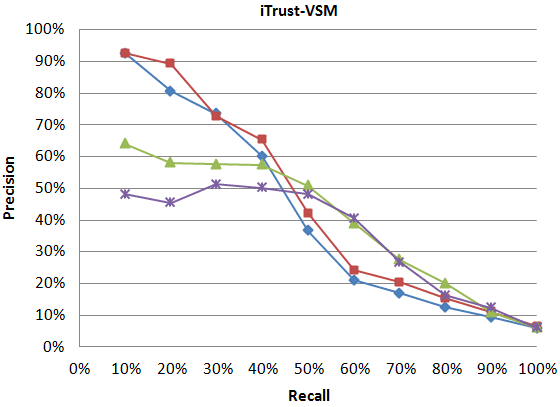
\includegraphics[width=0.31\textwidth,height=0.18\textheight]{figures/traceability_curves/iTrust_VSM.png}
   }
   \subfigure[ $iTrust_{JS}$ ]{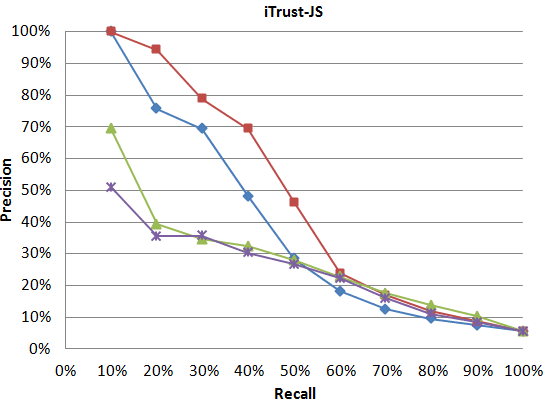
\includegraphics[width=0.31\textwidth,height=0.18\textheight]{figures/traceability_curves/iTrust_JS.png}
   }
   \subfigure[ $iTrust_{LSI}$ ]{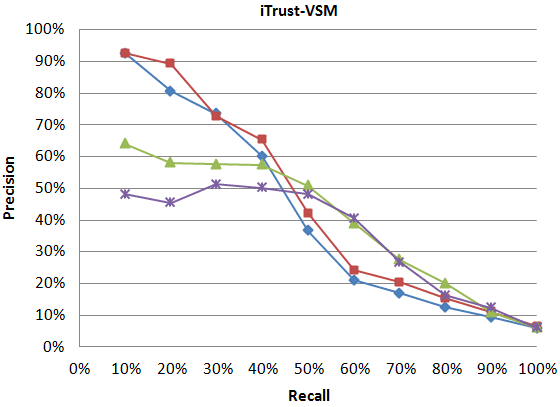
\includegraphics[width=0.31\textwidth,height=0.18\textheight]{figures/traceability_curves/iTrust_VSM.png}
   }
    \subfigure[ $Gantt_{VSM}$ ]{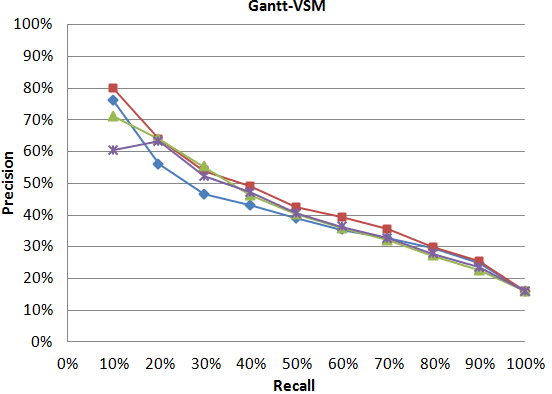
\includegraphics[width=0.31\textwidth,height=0.18\textheight]{figures/traceability_curves/Gantt_VSM.png}
   }
   \subfigure[ $Gantt_{JS}$ ]{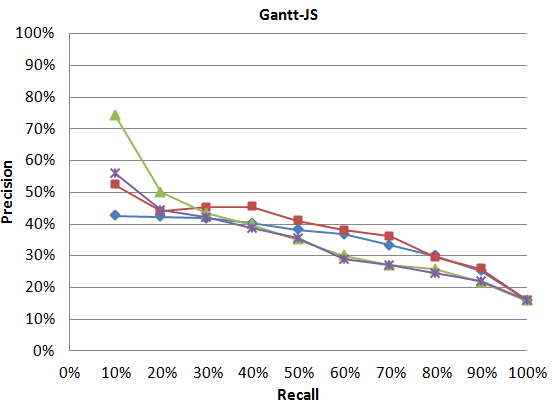
\includegraphics[width=0.31\textwidth,height=0.18\textheight]{figures/traceability_curves/Gantt_JS.png}
   }
   \subfigure[ $Gantt_{LSI}$ ]{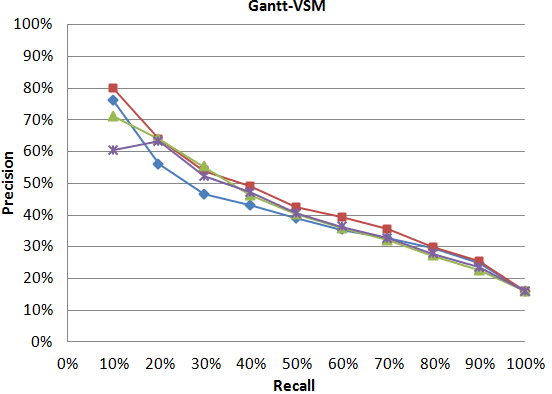
\includegraphics[width=0.31\textwidth,height=0.18\textheight]{figures/traceability_curves/Gantt_VSM.png}
   }
    \subfigure[ $jHotDraw_{VSM}$ ]{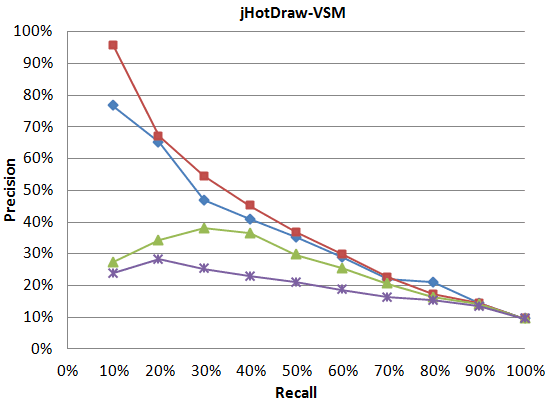
\includegraphics[width=0.31\textwidth,height=0.18\textheight]{figures/traceability_curves/jHotDraw_VSM.png}
   }
   \subfigure[ $jHotDraw_{JS}$ ]{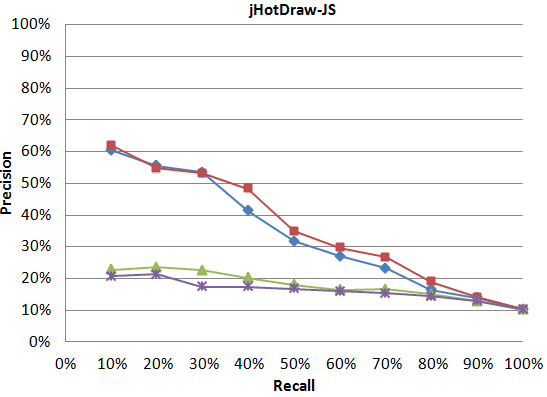
\includegraphics[width=0.31\textwidth,height=0.18\textheight]{figures/traceability_curves/jHotDraw_JS.png}
   }
   \subfigure[ $jHotDraw_{LSI}$ ]{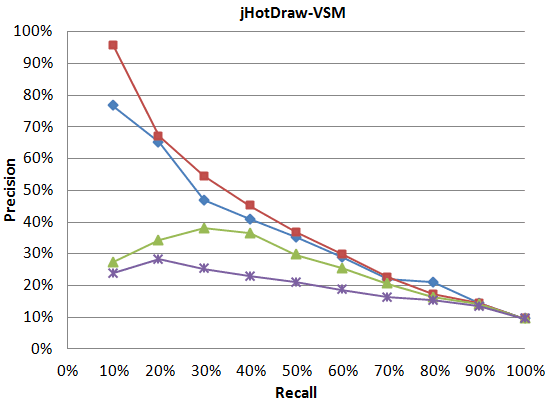
\includegraphics[width=0.31\textwidth,height=0.18\textheight]{figures/traceability_curves/jHotDraw_VSM.png}
   }
   \caption{F-measure/cut curves for iTrust, AquaLush and Connect between Release.}
   \label{fmeasure_release}
\end{figure*}

根据表N所示,我们发现O-CSTI与PageRank的表现并没有明显的优于IR-Only方法,因此我们主要关注于TRICE和IR-Only间的比较。表N展示了TRICE与IR-Only在不同的Recall水平上的AP与FP(False Positive),可以看出TRICE能够将检索的AP提高21.37\%(在Recall水平为40\%的iTrust-JS下),误报减少445(在Recall水平为80\%的iTrust-JS下)。同样,我们观察发现,TRICE方法几乎没有引入额外的误报,唯一的例外是在Recall水平为80\%的jHotDraw下,TRICE额外引入了185个FP。这些发现表明通过代码依赖关系的紧密度分析与重排序算法,追踪关系生成方法的效果能够被有效的提高,并且很少引入额外的误报。

\begin{table}[]
\centering
\caption{My caption}
\label{my-label}
\begin{tabular}{@{}cccccccccc@{}}
\toprule
         &     & \multicolumn{2}{c}{Recall (20\%)} & \multicolumn{2}{c}{Recall (40\%)} & \multicolumn{2}{c}{Recall (60\%)} & \multicolumn{2}{c}{Recall (80\%)} \\ \midrule
         &     & Precision          & FP           & Precision          & FP           & Precision          & FP           & Precision          & FP           \\
iTrust   & VSM & +8.64\%            & -6           & +5.12\%            & -13          & +3.00\%            & -89          & +2.74\%            & -280         \\
         & JS  & +18.58\%           & -13          & +21.37\%           & -64          & +5.76\%            & -196         & +2.57\%            & -445         \\
         & LSI & +1.46\%            & -1           & +4.52\%            & -12          & +3.40\%            & -86          & +4.39\%            & -425         \\
Gantt    & VSM & +7.86\%            & -14          & +6.03\%            & -36          & +3.81\%            & -52          & +0.62\%            & -28          \\
         & JS  & +1.75\%            & -6           & +5.33\%            & -37          & +1.11\%            & -15          & -0.46\%            & +13          \\
         & LSI & -1.94\%            & +3           & +2.92\%            & -20          & +3.24\%            & -45          & +2.63\%            & -83          \\
jHotDraw & VSM & +1.95\%            & -2           & +4.16\%            & -20          & +0.91\%            & -14          & -3.81\%            & +185         \\
         & JS  & -0.68\%            & +1           & +6.97\%            & -31          & +2.54\%            & -42          & +2.52\%            & -142         \\
         & LSI & -2.20\%            & +2           & +4.66\%            & -21          & +3.54\%            & -51          & +0.23\%            & -12          \\ \bottomrule
\end{tabular}
\end{table}

根据实验结果,我们还有一点额外的观察。如果基于信息检索生成的候选追踪关系质量较高(例如,iTrust-JS,反之,jHotDraw-VSM),则TRICE能够带来较大的提高。这表明TRICE能够获益于追踪关系的提高,甚至与其他改进方法相协作。

总体上来说,实验结果表明代码依赖关系的紧密度分析能够帮助提高基于信息检索的追踪关系生成方法的精度,当Recall水平在20\%至80\%时,提升较为明显。

\section{本章小结}

在本章中,我们提出了一种代码依赖关系的紧密度分析方法以量化代码类之间依赖的交互程度。同时,基于代码关系的紧密度分析,我们提出了一种改进的需求到代码间追踪关系的生成方法TRICE,并在三个真实的软件系统中设计并完成了实验,以证明TRICE的有效性。

% \bibliography{reference}